\chapter{Обзор соревновательных дисциплин}
{\bfseries Анонс:}\\\\
Обзор основных соревновательных дисциплин. Проекты на Lego Mindstorms. Обзор платформы Arduino.\\\\
{\bfseries Цели:}
\begin{itemize}
	\item{}{\bfseries Обучающие:} Ознакомить с основными направлениями школьной робототехники следующей ступени.   
	\item{}{\bfseries Развивающая:} Развитие познавательного интереса учащихся.\\
\end{itemize}	
{\bfseries Ход занятия:}\\\\
\begin{tabular}[h!]{lll}
	{\hyperlink{lesson30x1}{1. Организационный момент}}&{Презентация}&{(15 мин)}\\
	{\hyperlink{lesson30x2}{2. Лего-проекты}}&{Презентация}&{(15 мин)}\\
	{\hyperlink{lesson30x3}{3. Лего-соревнования}}&{Презентация}&{(25 мин)}\\
	{\hyperlink{lesson30x4}{4. Соревнования FTC FIRST}}&{Презентация}&{(25 мин)}\\
	{\hyperlink{lesson30x5}{5. Проекты на Arduino}}&{Презентация}&{(25 мин)}\\
\end{tabular}\\\\

{\hypertarget{lesson30x1}{\blackBlueText{I. Организационный момент}}}\\\\	

Итак, первые шаги сделаны. Закономерный вопрос «Что дальше?». Этому и будет посвящено последнее занятие.

{\slshape В зависимости от конкретной ситуации для учащихся тему можно переформулировать по разному: «обзор спецкурсов следующего уровня», «течения школьной робототехники», «чем заняться летом» и тп. В случае если в учебном заведении дальше реализуется только одна конкретная программа можно подробнее осветить ее.}

Во-первых, это стандартные соревнования  городского и всероссийского уровня. Краткий обзор соревновательных дисциплин будет произведен ниже, но так же каждый год появляются какие-то новые дисциплины и усложняются некоторые старые. Участие в соревнованиях крайне рекомендовано по мере дальнейшего роста юных робототехников. Это позволяет увеличить мотивированность учащихся, научить их работать в сжатые сроки, повысить их коммуникативные навыки. Дети начинают чувствовать себя частью глобального робототехнического сообщества, общаются со сверстниками, происходит обмен идеями, оценка собственного труда и достижений. Так же обретают весомость выражения « в сжатые сроки», «прочная конструкция», «калибровка освещенности» и тп. Большинство подобных вопросов были освещены в рамках данного курса, но одно дело проверять в классе прочность своего робота, и совсем другое~--- видеть как уплывает призовое место из-за неукрепленной балки, из-за плохо подобранного коэффициента. И лишь поучаствовав в паре-тройке фестивалей, усовершенствовав своего робота, написав по нему документацию и передав ее новому поколению кружковцев, ребенок в полной мере ощущает важность своего труда и необходимость ведения записей о своей работе.

Во-вторых, это конференции и чтения разных уровней. Опять же, одно дело создать свой маленький проект и защитить его в школьном сообществе и совсем другое~--- выступить перед незнакомой аудиторией, хотя бы на районном уровне. Помимо страха публичных выступлений дети сталкиваются с проблемой непонимания. Вещи, казавшиеся им самоочевидными, им проработавшим над этим проектом полтора--два месяца, оказываются совершенно непонятны посторонним людям без должного объяснения. Говорить так, что бы тебя поняли, это ценнейшее умение, которое не приобрести без должной практики. Кроме этого на конференциях разумеется так же происходит обмен информацией между участниками, одним словом «себя показать, других посмотреть» это необходимая часть учебного процесса.\\\\

{\hypertarget{lesson30x2}{\blackBlueText{II. Лего-проекты}}}\\\\

До сих пор речь шла о новых формах работы, но платформа оставалась той же~--- Lego Mindstorms NXT 2.0. Как мы убедились, она отлично подходит для первых шагов в робототехнике, но можно ли сделать что-то «серьезное», сложный проект на базе детского конструктора? Оказывается, да, все ограничено лишь фантазией.
\clearpage
В Интернете можно найти роботов, собирающих кубик рубика.

\begin{figure}[h!]
	\begin{center}
		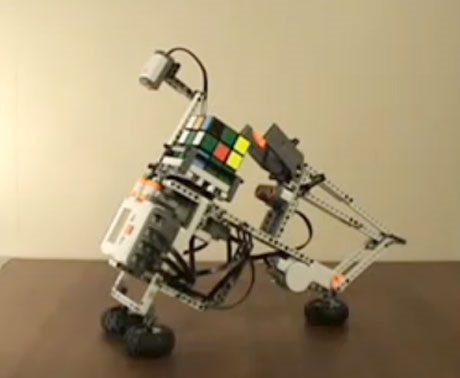
\includegraphics[width=0.83\linewidth]{chapters/chapter30/images/1}
		\caption{}
		\label{ris:image30x1}
	\end{center}
\end{figure}

Роботов, решающих судоку

\begin{figure}[h!]
	\begin{center}
		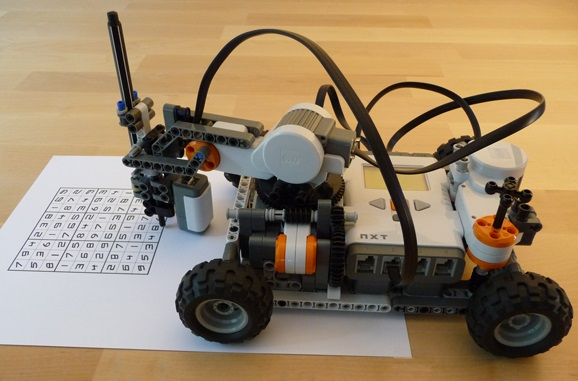
\includegraphics[width=0.83\linewidth]{chapters/chapter30/images/2}
		\caption{}
		\label{ris:image30x2}
	\end{center}
\end{figure}

Роботов, рисующих картины

\begin{figure}[h!]
	\begin{center}
		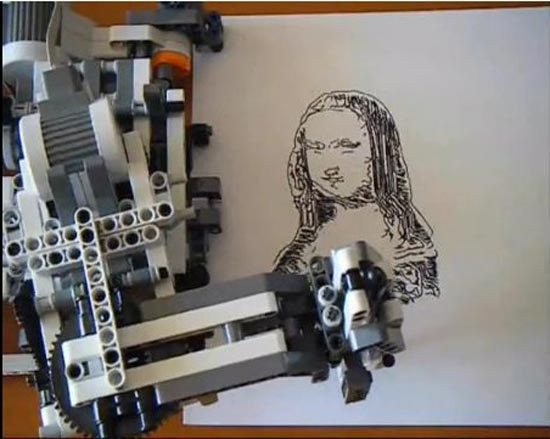
\includegraphics[width=0.83\linewidth]{chapters/chapter30/images/3}
		\caption{}
		\label{ris:image30x3}
	\end{center}
\end{figure}

Роботов-шахматные фигуры, самостоятельно двигающихся и думающих:

\begin{figure}[h!]
	\begin{center}
		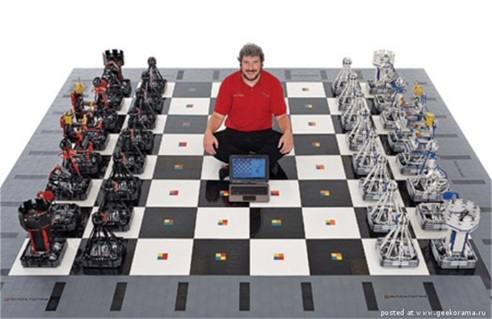
\includegraphics[width=0.83\linewidth]{chapters/chapter30/images/4}
		\caption{}
		\label{ris:image30x4}
	\end{center}
\end{figure}

И все из Лего! Поэтому списывать конструктор как «детский», «для начинающих», безусловно рано, множество интересных проектов более высокого уровня, чем финальные проекты этой ступени, могут быть реализованы всеми желающими. Команды из России регулярно занимают призовые места на международных конкурсах творческих Лего проектов, так что определенно творческому человеку есть куда расти в данном направлении.\\\\

{\hypertarget{lesson30x3}{\blackBlueText{III. Лего-соревнования}}}\\\\

Кратко рассмотрим наиболее часто встречающиеся на всероссийских и региональных турнирах дисциплины.\\\\

Группа соревнований «Линия»

\begin{itemize}
	\item Следование по линии
	\item Линия профи
	\item Дорога
	\item Слалом
	\item Инверсная линия
	\item Линия-пазл
\end{itemize}

С основной идеей этих соревнований мы уже знакомы. В простейшей вариации (Следование по линии)  робот должен за кратчайшее время проехать по извилистой черной линии на белом фоне. Один из самых популярных соревновательных видов, собирает сотни участников,  традиционно является первыми соревнованиями для самых маленьких.  Некоторые варианты правил ограничивают участников использованием только наборов Лего, в других~--- допустимы «самодельные» роботы. Сделать робота, который лучше всех справиться с задачей – трудно; робота, который просто справится с задачей~--- доступно любому. Поэтому с годами начали появляться усложненные варианты: часть линии заменена на пунктир (Линия-профи); по линии ездит помеха, которую необходимо объехать (Дорога); помехи надо объезжать слева и справа по очереди (Слалом); инверсия цветов поле-линия (Инверсная линия), наличие перекрестков (Линия пазл). В усложненных видах участвует на порядок меньше людей, с выполнением задачи справляются немногие. Хочется так же отметить, что  усложняется программная часть задачи, конструкции не претерпевают значительных изменений и обычно представляет собой модификацию стандартной трехколесной тележки.\\\\

Другая ветвь соревнований, типа Линия, с усложненной конструкционной частью:

\begin{itemize}
	\item Лестница
	\item Стена
\end{itemize}

В соревнованиях Лестница, робот должен проехать по линии, нарисованной на ступенях разной высоты.  Сложности в реализации вызывает все: подъем на ступень, спуск с нее, не потерять при этом линию. Достаточно сказать, что за 3 года существования дисциплины только один раз одна команда преодолела целиком всю дистанцию. 

Соревнования Стена заключаются в преодолении роботом вертикальной стенки высотой в 30 см, находящейся на линии. В текущей редакции правил линия прямая и движение по ней не представляет никакого труда, в то время как конструкционная часть задачи очень сложна.\\\\

Группа соревнований кегельринг:

\begin{itemize}
	\item Кегельринг
	\item Кегельринг-макро
\end{itemize}

В соревнованиях Кегельринг робот находится в белом круге, ограниченном черной  линией. Внутри круга находится некоторое количество банок, которые робот должен вытолкнуть из круга за наименьшее время. За банки, оставшиеся внутри круга, начисляется штраф. Два стандартных способа решения: проезд робота по спирали, заметающий всю площадь круга либо поиск банок при помощи сонара и выталкивание их по одной. Соревнования Кегельринг-макро представляют собой чуть усложненную версию: банки бывают двух цветов и выталкивать надо лишь банки одного, определенного цвета. 

Отметим, что несмотря на важность отдельных моментов конструкции (расположение сенсоров и бампера для выталкивания) основным в задаче Кегельринг–макро так же является вопрос программирования.\\\\

Группа соревнований сумо:

\begin{itemize}
	\item Механическое сумо
	\item Интеллектуальное сумо
	\item Мини-сумо
	\item Микро-сумо
\end{itemize}

С концепцией соревнований Сумо читатели уже знакомы. Роботы должны перетолкать друг друга, кто первый оказался за пределами очерченного круга – тот проиграл. В обычном сумо роботы приходят в контакт и, не разрывая его, толкаются. В интеллектуальном робот может уклоняться и искать соперника при помощи датчиков. Мини-сумо названо так, потому что разрешенные размеры роботов меньше самого блока NXT, и в этой категории невозможно участвовать Лего-роботам.

Эта соревновательная дисциплина по большей части инженерная, т.к. победа зависит от правильно подобранного передаточного соотношения, распределения массы робота, борьбы с поддеванием, выключением и тп.\\\\

\begin{itemize}
	\item Лабиринт
\end{itemize}

Роботу надо проехать через лабиринт от входа до выхода. В существующей редакции правил лабиринт односвязен, поэтому его можно пройти, пользуясь правилом правой руки (все время следовать, держась за правую стенку). Задача напоминает «Движение вдоль стенки», но на крутых 90 градусных поворотах робот все время вылетает, что и представляет основную техническую трудность задачи. 

В данном соревновании удачно сочетаются сложные инженерные и программные проблемы.\\\\

\begin{itemize}
	\item Управляемый футбол
	\item Автономный футбол
\end{itemize}

Главная игра планеты не могла не найти своего отражения в робототехнике. В управляемом футболе, команда роботов составом от 3 до 5 игроков играет под управлением операторов на поле 7 на 5 метров. В автономном виде запрещено управлять роботом, они должны мыслить и принимать решения самостоятельно, общаясь друг с другом (в команде не более двух роботов) и отслеживая мяч, с инфракрасным маячком внутри.\\\\

{\hypertarget{lesson30x4}{\blackBlueText{IV. Соревнования FTC FIRST}}}\\\\

Отдельно хочется поговорить о соревнованиях FTC FIRST. Их особенность в том, что это и немножко творческий проект, и безусловно, соревнования, и что самое ценное, это соревнования с приставкой «инженерные». 

Сами соревнования родом из США и имеют там бешенную популярность. Последние несколько лет множество других стран присоединилось к движению FTC, в том числе и Россия.

В начале сентября на официальном сайте вывешиваются правила игр на этот год, по этим правилам команды будут играть весь сезон, вплоть до международного финала в апреле. Робот каждый год собирается из одного и того же набора, выпускаемого так же фирмой Лего, плюс допустимо использовать любые детали и механизмы не фабричного производства. Мозгом робота является все тот же хорошо знакомый нам блок Lego Mindstorms NXT 2.0. Правила игры всегда довольно запутаны и предполагают решение целого ряда инженерных задач. Так, в сезоне 2012-2013 робот должен был уметь вешать кольца на крючки разного уровня, забираться на небольшую платформу, распознавать вес колец, неотличимых внешне, уметь действовать автономно и управляемо, искать инфракрасный маячок и ориентироваться по нему, поднимать союзника над землей. Существенно, что для победы в игре е обязательно реализовать все возможные действия робота, грамотная стратегия и работа в альянсе с союзником тоже играет немаловажную роль. Но самым главным отличием от большинства робототехнических соревнований, является момент наличия и защиты технической книги. Компетентное жюри выслушивает каждую команду и подробно расспрашивает ее о технических решениях, придуманных ими, о пути пройденном командой в течение сезона. Награды даются как за победы в играх, так и за лучшую техническую книгу, за лучшее взаимодействие с другими командами, за лучший дизайн и другие важные достижения.

В США практически в каждой школе есть своя команда, каждый год на уровне округов, затем штатов проводятся отборочные соревнования, затем команды выходят в финал. В России в последние годы на фестивале РобоФест проводятся отборочные соревнования на всероссийском уровне, а победители получают возможность поучаствовать в международном финале.

Соревнования FIRST FTC допускают к участию детей в возрасте от 14 до 18 лет.\\\\

{\hypertarget{lesson30x5}{\blackBlueText{V. Проекты Arduino}}}\\\\

В заключение, отвлечемся от различных Лего соревнований и кратко обрисуем самую популярную «взрослую» платформу для создания различных роботов. Это Arduino~--- небольшая плата, размером со спичечный коробок. Идейно, это тот же самый «мозг» робота, как известный нам блок Лего, но меньших размеров и больших возможностей. На плате укреплен процессор, память, а так же есть пара десятков контактов, к которым можно подключать всевозможные устройства и платы (датчики, моторы, лампочки, роутеры, сотовые антенны\dots).
\clearpage
\begin{figure}[h!]
	\begin{center}
		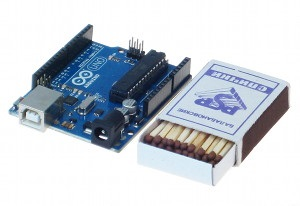
\includegraphics[width=0.76\linewidth]{chapters/chapter30/images/5}
		\caption{}
		\label{ris:image30x5}
	\end{center}
\end{figure}

В принципе суть работы с  Arduino точно такая же, как с набором Lego Mindstorms NXT 2.0. В процессор с компьютера загружается программа, которую так же можно писать на С/С++, только сама среда разработки немного другая чем для Лего (Arduino IDE). Еще одно достоинство в том что эта среда в отличие от RobotC бесплатна. 

Процессор в соответствии с заданной программой будет управлять всей подключенной электроникой, согласно задумке автора. На плату Arduino так же можно ставить множество так называемых «шилдов» (shields), т.е. плат расширения. существуют платы расширения для подключения к локальной сети и интернету, для управления мощными моторами, для получения координат и времени со спутников GPS  и многие другие. Подобрать необходимые компоненты, немного знаний по электронике и вы можете собирать любые мыслимые и немыслимые гаджеты. 

Умный дом~--- это дело далекого будущего? За несколько месяцев можно автоматизировать практически все своими руками. Датчик температуры передает плате показания о температуре в комнатах, она пересылает эти данные хозяину. Он по SMS отдаете команду~--- и вот уже в спальне поддерживается заданная температура. Подсветить ступеньки на темной лестнице? Пожалуйста!\\
\href{http://arduino-projects.ru/projects/podsvetka-lestnitsyi-s-pomoschyu-arduino/}{\whiteBlueText{\slshape http://arduino-projects.ru/projects/podsvetka-lestnitsyi-s-pomoschyu-arduino/}}

Любители музыки  создают современную версию музыкальных инструментов~--- лазерную арфу:\\
\href{http://arduino-projects.ru/projects/lazernaya-arfa/}{\whiteBlueText{\slshape http://arduino-projects.ru/projects/lazernaya-arfa/}}

А домашнего любимца покормит по часам автоматическая кормушка:\\
\href{http://arduino-projects.ru/projects/kormyozhka-sobaki-cherez-tvitter/}{\whiteBlueText{\slshape http://arduino-projects.ru/projects/kormyozhka-sobaki-cherez-tvitter/}}

Так что дальше еще много всего интересного и длинный путь ребенка в «настоящую» робототехнику. Или будущее уже наступило?
